% Created by tikzDevice version 0.12.6 on 2024-02-26 07:48:49
% !TEX encoding = UTF-8 Unicode
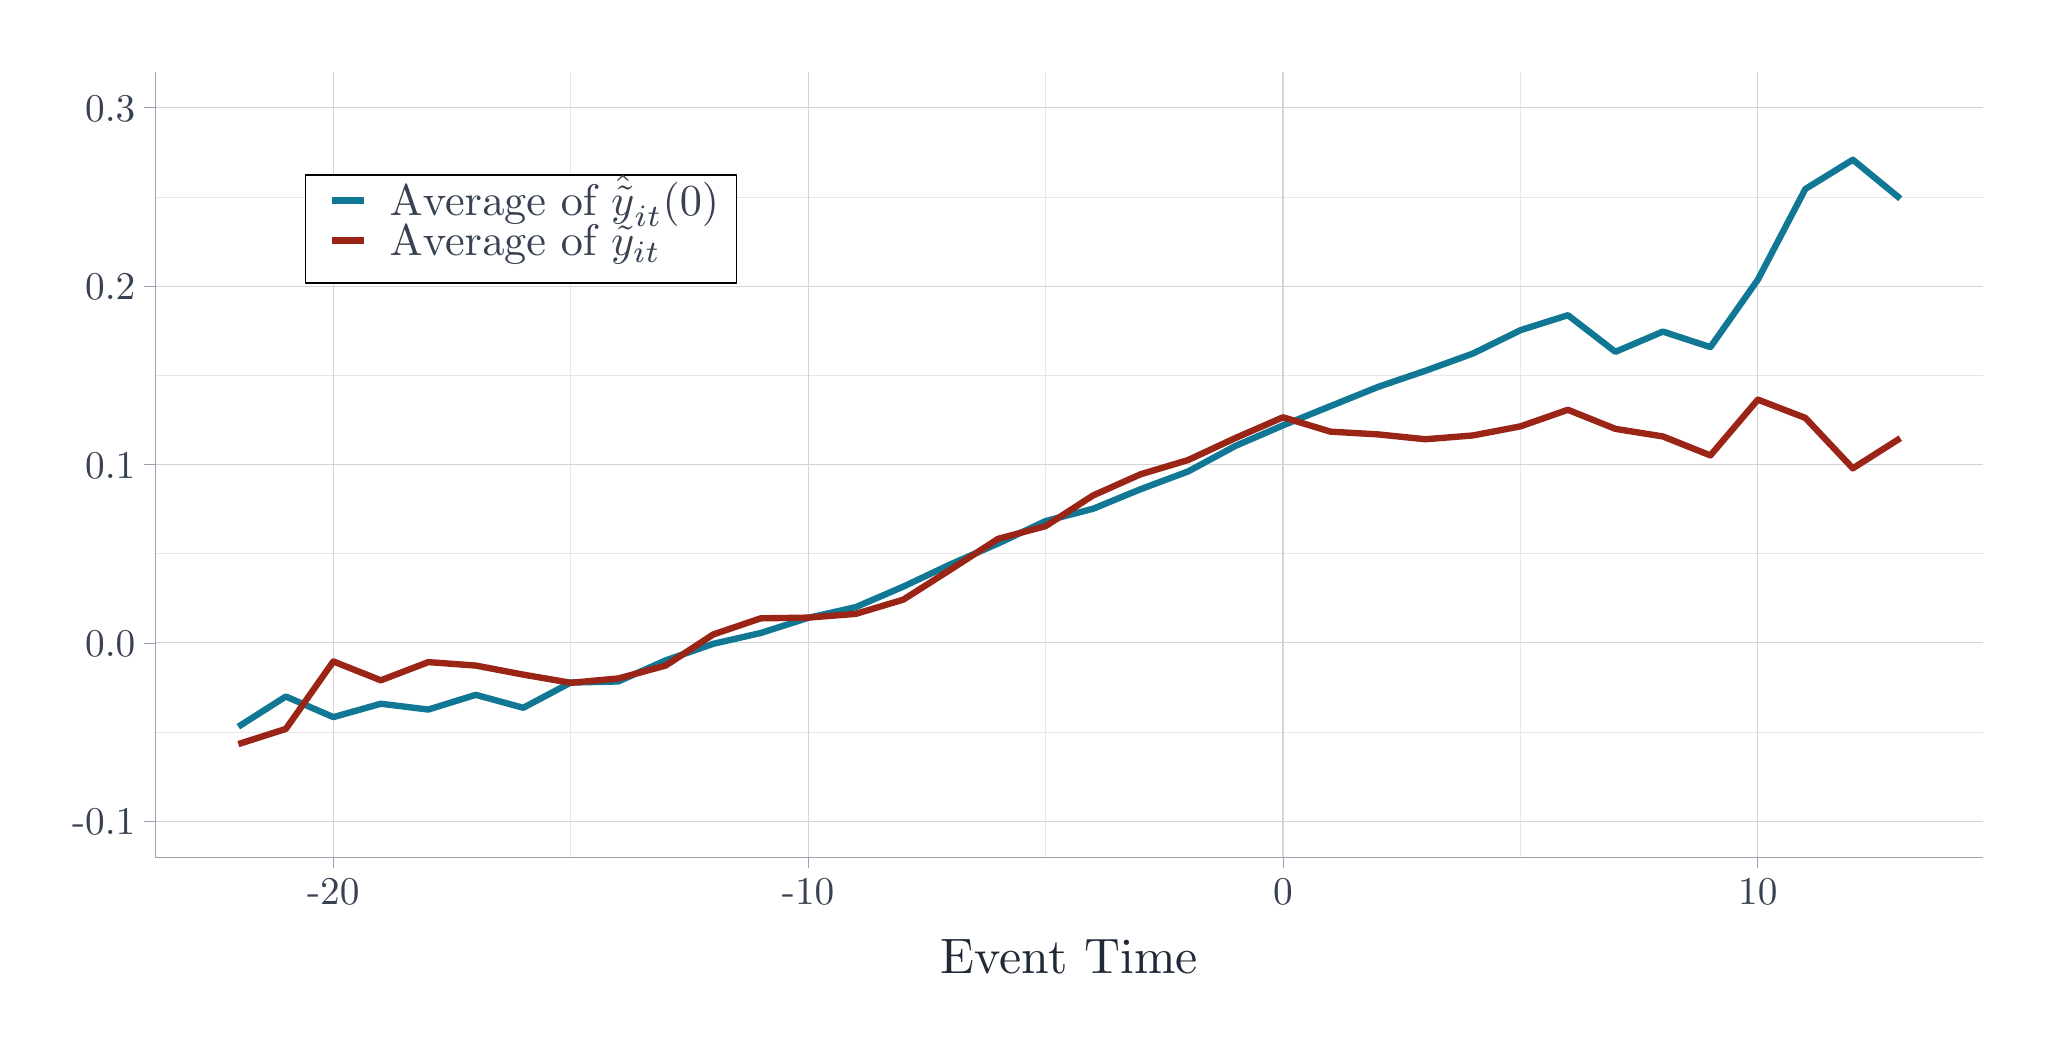
\begin{tikzpicture}[x=1pt,y=1pt]
\definecolor{fillColor}{RGB}{255,255,255}
\path[use as bounding box,fill=fillColor] (0,0) rectangle (722.70,361.35);
\begin{scope}
\path[clip] (  0.00,  0.00) rectangle (722.70,361.35);
\definecolor{drawColor}{RGB}{255,255,255}

\path[draw=drawColor,line width= 0.8pt,line join=round,line cap=round,fill=fillColor] (  0.00,  0.00) rectangle (722.70,361.35);
\end{scope}
\begin{scope}
\path[clip] ( 46.10, 61.65) rectangle (706.70,345.35);
\definecolor{drawColor}{RGB}{255,255,255}
\definecolor{fillColor}{RGB}{255,255,255}

\path[draw=drawColor,line width= 0.8pt,line join=round,line cap=round,fill=fillColor] ( 46.10, 61.65) rectangle (706.70,345.35);
\definecolor{drawColor}{RGB}{229,231,235}

\path[draw=drawColor,line width= 0.2pt,line join=round] ( 46.10,106.79) --
	(706.70,106.79);

\path[draw=drawColor,line width= 0.2pt,line join=round] ( 46.10,171.26) --
	(706.70,171.26);

\path[draw=drawColor,line width= 0.2pt,line join=round] ( 46.10,235.74) --
	(706.70,235.74);

\path[draw=drawColor,line width= 0.2pt,line join=round] ( 46.10,300.22) --
	(706.70,300.22);

\path[draw=drawColor,line width= 0.2pt,line join=round] (196.24, 61.65) --
	(196.24,345.35);

\path[draw=drawColor,line width= 0.2pt,line join=round] (367.82, 61.65) --
	(367.82,345.35);

\path[draw=drawColor,line width= 0.2pt,line join=round] (539.41, 61.65) --
	(539.41,345.35);
\definecolor{drawColor}{RGB}{209,213,219}

\path[draw=drawColor,line width= 0.4pt,line join=round] ( 46.10, 74.55) --
	(706.70, 74.55);

\path[draw=drawColor,line width= 0.4pt,line join=round] ( 46.10,139.03) --
	(706.70,139.03);

\path[draw=drawColor,line width= 0.4pt,line join=round] ( 46.10,203.50) --
	(706.70,203.50);

\path[draw=drawColor,line width= 0.4pt,line join=round] ( 46.10,267.98) --
	(706.70,267.98);

\path[draw=drawColor,line width= 0.4pt,line join=round] ( 46.10,332.45) --
	(706.70,332.45);

\path[draw=drawColor,line width= 0.4pt,line join=round] (110.45, 61.65) --
	(110.45,345.35);

\path[draw=drawColor,line width= 0.4pt,line join=round] (282.03, 61.65) --
	(282.03,345.35);

\path[draw=drawColor,line width= 0.4pt,line join=round] (453.61, 61.65) --
	(453.61,345.35);

\path[draw=drawColor,line width= 0.4pt,line join=round] (625.20, 61.65) --
	(625.20,345.35);
\definecolor{drawColor}{RGB}{16,120,149}

\path[draw=drawColor,line width= 2.3pt,line join=round] ( 76.13,108.76) --
	( 93.29,119.67) --
	(110.45,112.21) --
	(127.61,117.05) --
	(144.76,114.95) --
	(161.92,120.27) --
	(179.08,115.59) --
	(196.24,124.70) --
	(213.40,125.10) --
	(230.56,132.73) --
	(247.71,138.70) --
	(264.87,142.61) --
	(282.03,148.09) --
	(299.19,151.95) --
	(316.35,159.35) --
	(333.51,167.45) --
	(350.66,174.95) --
	(367.82,183.07) --
	(384.98,187.50) --
	(402.14,194.57) --
	(419.30,200.98) --
	(436.46,210.23) --
	(453.61,217.64) --
	(470.77,224.60) --
	(487.93,231.53) --
	(505.09,237.38) --
	(522.25,243.60) --
	(539.41,252.03) --
	(556.56,257.46) --
	(573.72,244.21) --
	(590.88,251.53) --
	(608.04,245.91) --
	(625.20,270.29) --
	(642.36,303.05) --
	(659.51,313.63) --
	(676.67,299.56);
\definecolor{drawColor}{RGB}{154,36,21}

\path[draw=drawColor,line width= 2.3pt,line join=round] ( 76.13,102.47) --
	( 93.29,107.95) --
	(110.45,132.33) --
	(127.61,125.52) --
	(144.76,132.09) --
	(161.92,130.85) --
	(179.08,127.57) --
	(196.24,124.62) --
	(213.40,126.18) --
	(230.56,130.85) --
	(247.71,142.09) --
	(264.87,147.91) --
	(282.03,148.17) --
	(299.19,149.52) --
	(316.35,154.64) --
	(333.51,165.54) --
	(350.66,176.64) --
	(367.82,181.22) --
	(384.98,192.32) --
	(402.14,199.96) --
	(419.30,205.10) --
	(436.46,213.09) --
	(453.61,220.56) --
	(470.77,215.37) --
	(487.93,214.38) --
	(505.09,212.62) --
	(522.25,214.00) --
	(539.41,217.28) --
	(556.56,223.27) --
	(573.72,216.37) --
	(590.88,213.64) --
	(608.04,206.78) --
	(625.20,226.95) --
	(642.36,220.34) --
	(659.51,202.11) --
	(676.67,213.01);

\path[] ( 46.10, 61.65) rectangle (706.70,345.35);
\end{scope}
\begin{scope}
\path[clip] (  0.00,  0.00) rectangle (722.70,361.35);
\definecolor{drawColor}{RGB}{156,163,175}

\path[draw=drawColor,line width= 0.3pt,line join=round] ( 46.10, 61.65) --
	( 46.10,345.35);
\end{scope}
\begin{scope}
\path[clip] (  0.00,  0.00) rectangle (722.70,361.35);
\definecolor{drawColor}{RGB}{55,65,81}

\node[text=drawColor,anchor=base east,inner sep=0pt, outer sep=0pt, scale=  1.42] at ( 38.90, 69.65) {-0.1};

\node[text=drawColor,anchor=base east,inner sep=0pt, outer sep=0pt, scale=  1.42] at ( 38.90,134.13) {0.0};

\node[text=drawColor,anchor=base east,inner sep=0pt, outer sep=0pt, scale=  1.42] at ( 38.90,198.61) {0.1};

\node[text=drawColor,anchor=base east,inner sep=0pt, outer sep=0pt, scale=  1.42] at ( 38.90,263.08) {0.2};

\node[text=drawColor,anchor=base east,inner sep=0pt, outer sep=0pt, scale=  1.42] at ( 38.90,327.56) {0.3};
\end{scope}
\begin{scope}
\path[clip] (  0.00,  0.00) rectangle (722.70,361.35);
\definecolor{drawColor}{RGB}{156,163,175}

\path[draw=drawColor,line width= 0.3pt,line join=round] ( 42.10, 74.55) --
	( 46.10, 74.55);

\path[draw=drawColor,line width= 0.3pt,line join=round] ( 42.10,139.03) --
	( 46.10,139.03);

\path[draw=drawColor,line width= 0.3pt,line join=round] ( 42.10,203.50) --
	( 46.10,203.50);

\path[draw=drawColor,line width= 0.3pt,line join=round] ( 42.10,267.98) --
	( 46.10,267.98);

\path[draw=drawColor,line width= 0.3pt,line join=round] ( 42.10,332.45) --
	( 46.10,332.45);
\end{scope}
\begin{scope}
\path[clip] (  0.00,  0.00) rectangle (722.70,361.35);
\definecolor{drawColor}{RGB}{156,163,175}

\path[draw=drawColor,line width= 0.3pt,line join=round] ( 46.10, 61.65) --
	(706.70, 61.65);
\end{scope}
\begin{scope}
\path[clip] (  0.00,  0.00) rectangle (722.70,361.35);
\definecolor{drawColor}{RGB}{156,163,175}

\path[draw=drawColor,line width= 0.3pt,line join=round] (110.45, 57.65) --
	(110.45, 61.65);

\path[draw=drawColor,line width= 0.3pt,line join=round] (282.03, 57.65) --
	(282.03, 61.65);

\path[draw=drawColor,line width= 0.3pt,line join=round] (453.61, 57.65) --
	(453.61, 61.65);

\path[draw=drawColor,line width= 0.3pt,line join=round] (625.20, 57.65) --
	(625.20, 61.65);
\end{scope}
\begin{scope}
\path[clip] (  0.00,  0.00) rectangle (722.70,361.35);
\definecolor{drawColor}{RGB}{55,65,81}

\node[text=drawColor,anchor=base,inner sep=0pt, outer sep=0pt, scale=  1.42] at (110.45, 44.66) {-20};

\node[text=drawColor,anchor=base,inner sep=0pt, outer sep=0pt, scale=  1.42] at (282.03, 44.66) {-10};

\node[text=drawColor,anchor=base,inner sep=0pt, outer sep=0pt, scale=  1.42] at (453.61, 44.66) {0};

\node[text=drawColor,anchor=base,inner sep=0pt, outer sep=0pt, scale=  1.42] at (625.20, 44.66) {10};
\end{scope}
\begin{scope}
\path[clip] (  0.00,  0.00) rectangle (722.70,361.35);
\definecolor{drawColor}{RGB}{31,41,55}

\node[text=drawColor,anchor=base,inner sep=0pt, outer sep=0pt, scale=  1.80] at (376.40, 19.50) {Event Time};
\end{scope}
\begin{scope}
\path[clip] (  0.00,  0.00) rectangle (722.70,361.35);
\definecolor{drawColor}{RGB}{0,0,0}
\definecolor{fillColor}{RGB}{255,255,255}

\path[draw=drawColor,line width= 0.6pt,line join=round,line cap=round,fill=fillColor] (100.36,269.16) rectangle (256.09,308.06);
\end{scope}
\begin{scope}
\path[clip] (  0.00,  0.00) rectangle (722.70,361.35);
\definecolor{drawColor}{RGB}{255,255,255}
\definecolor{fillColor}{RGB}{255,255,255}

\path[draw=drawColor,line width= 0.8pt,line join=round,line cap=round,fill=fillColor] (108.36,291.61) rectangle (122.81,306.06);
\end{scope}
\begin{scope}
\path[clip] (  0.00,  0.00) rectangle (722.70,361.35);
\definecolor{drawColor}{RGB}{16,120,149}

\path[draw=drawColor,line width= 2.3pt,line join=round] (109.81,298.84) -- (121.37,298.84);
\end{scope}
\begin{scope}
\path[clip] (  0.00,  0.00) rectangle (722.70,361.35);
\definecolor{drawColor}{RGB}{255,255,255}
\definecolor{fillColor}{RGB}{255,255,255}

\path[draw=drawColor,line width= 0.8pt,line join=round,line cap=round,fill=fillColor] (108.36,277.16) rectangle (122.81,291.61);
\end{scope}
\begin{scope}
\path[clip] (  0.00,  0.00) rectangle (722.70,361.35);
\definecolor{drawColor}{RGB}{154,36,21}

\path[draw=drawColor,line width= 2.3pt,line join=round] (109.81,284.38) -- (121.37,284.38);
\end{scope}
\begin{scope}
\path[clip] (  0.00,  0.00) rectangle (722.70,361.35);
\definecolor{drawColor}{RGB}{55,65,81}

\node[text=drawColor,anchor=base west,inner sep=0pt, outer sep=0pt, scale=  1.60] at (130.81,293.33) {Average of $\hat{\tilde{y}}_{it}(0)$};
\end{scope}
\begin{scope}
\path[clip] (  0.00,  0.00) rectangle (722.70,361.35);
\definecolor{drawColor}{RGB}{55,65,81}

\node[text=drawColor,anchor=base west,inner sep=0pt, outer sep=0pt, scale=  1.60] at (130.81,278.87) {Average of $\tilde{y}_{it}$};
\end{scope}
\end{tikzpicture}
